\documentclass[border=8pt,tikz]{standalone}
\usetikzlibrary{arrows.meta}
\tikzset{
    arrow shift factor/.initial=.5, % arrow shift option
    pics/arrow/.style={
        /tikz/sloped, /tikz/allow upside down,
        % /tikz/sloped用于让arrow与路径方向平行
        % /tikz/allow upside down关闭tikz自动调整side的功能
        setup code=\pgfarrowtotallength{#1}\pgftransformxshift{(\pgfkeysvalueof{/tikz/arrow shift factor})*\csname pgf@x\endcsname},%基于pgf提供的\pgfarrowdraw控制箭头
        code=\pgfarrowdraw{#1}}, 
      pics/arrow/.default=>,% handle设置默认值 .default
    } 
\begin{document}
    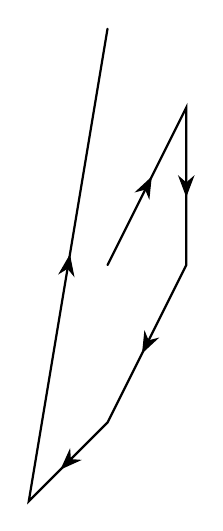
\begin{tikzpicture}[
            midwayarrow/.style={
            thick, cap=round,
            % every to句柄将自动合并在每个to(--)选项之后
            every to/.append style={edge node={pic[midway]{arrow={Stealth[scale=1.2]}}}}
        },]
        \draw[midwayarrow] (0,0) to (1,2) to (right:1) to (down:2) to ++(-1,-1) to (up:3);
    \end{tikzpicture}
\end{document}

